\documentclass[a4paper]{article}
\usepackage[warn]{mathtext}
\usepackage[utf8]{inputenc}
\usepackage[T2A]{fontenc}
\usepackage[english,russian]{babel}
\usepackage{multicol}
\usepackage{fancyhdr}
\usepackage{graphicx}
\usepackage{microtype}
\usepackage{wrapfig}
\usepackage{amsmath}
\usepackage{floatflt}
\usepackage{geometry} \geometry{verbose,a4paper,tmargin=2cm,bmargin=2cm,lmargin=1.5cm,rmargin=1.5cm}
\usepackage{float}
\usepackage{amssymb}
\usepackage{caption}
\usepackage{epsfig}
\usepackage{newunicodechar}

\begin{document}

\graphicspath{ {pic/} }
\begin{center}
    {\scshape\Large Лабораторная работа по твердотельной электронике} \par

    \

    {\huge\bfseries № 29: Исследование униполярных транзисторов с изолированным затвором} \par 

    \

    {\large Яромир Водзяновский Б04-852}
\end{center}

\

\

Будем исследовать нормально открытый $n$-канальный транзистор при положительных и отрицательных напряжениях на затворе.  

\begin{figure}[h]
    \begin{center}
    \begin{minipage}[h]{0.4\linewidth}
        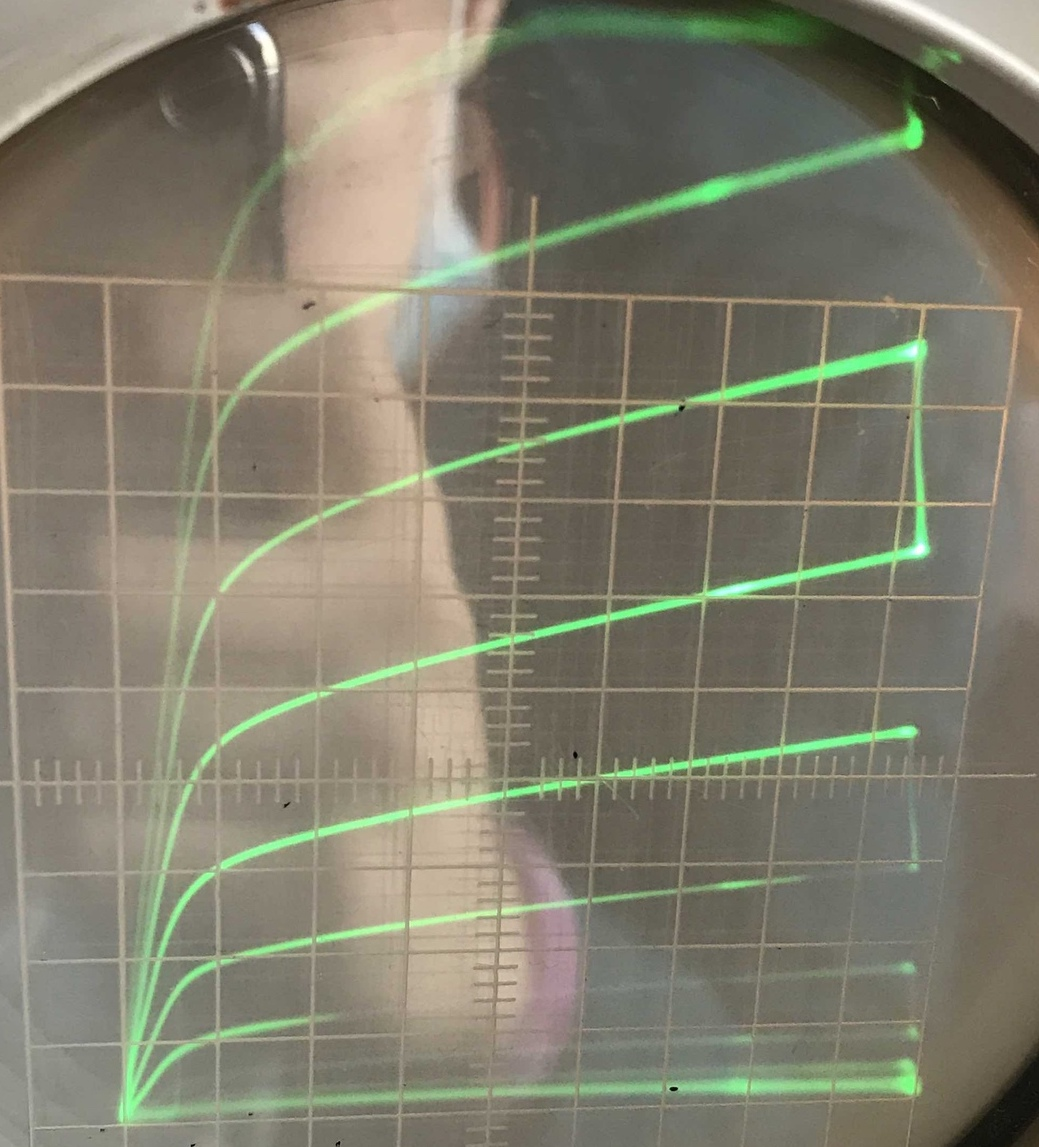
\includegraphics[width=1\linewidth]{p1.jpg}
        \caption{ВАХ при $V_з < 0$: X = +1 В, Y = +0.5 мА, Z = -0.2 В}
        \label{p1}
    \end{minipage}
    \hfill 
    \begin{minipage}[h]{0.4\linewidth}
        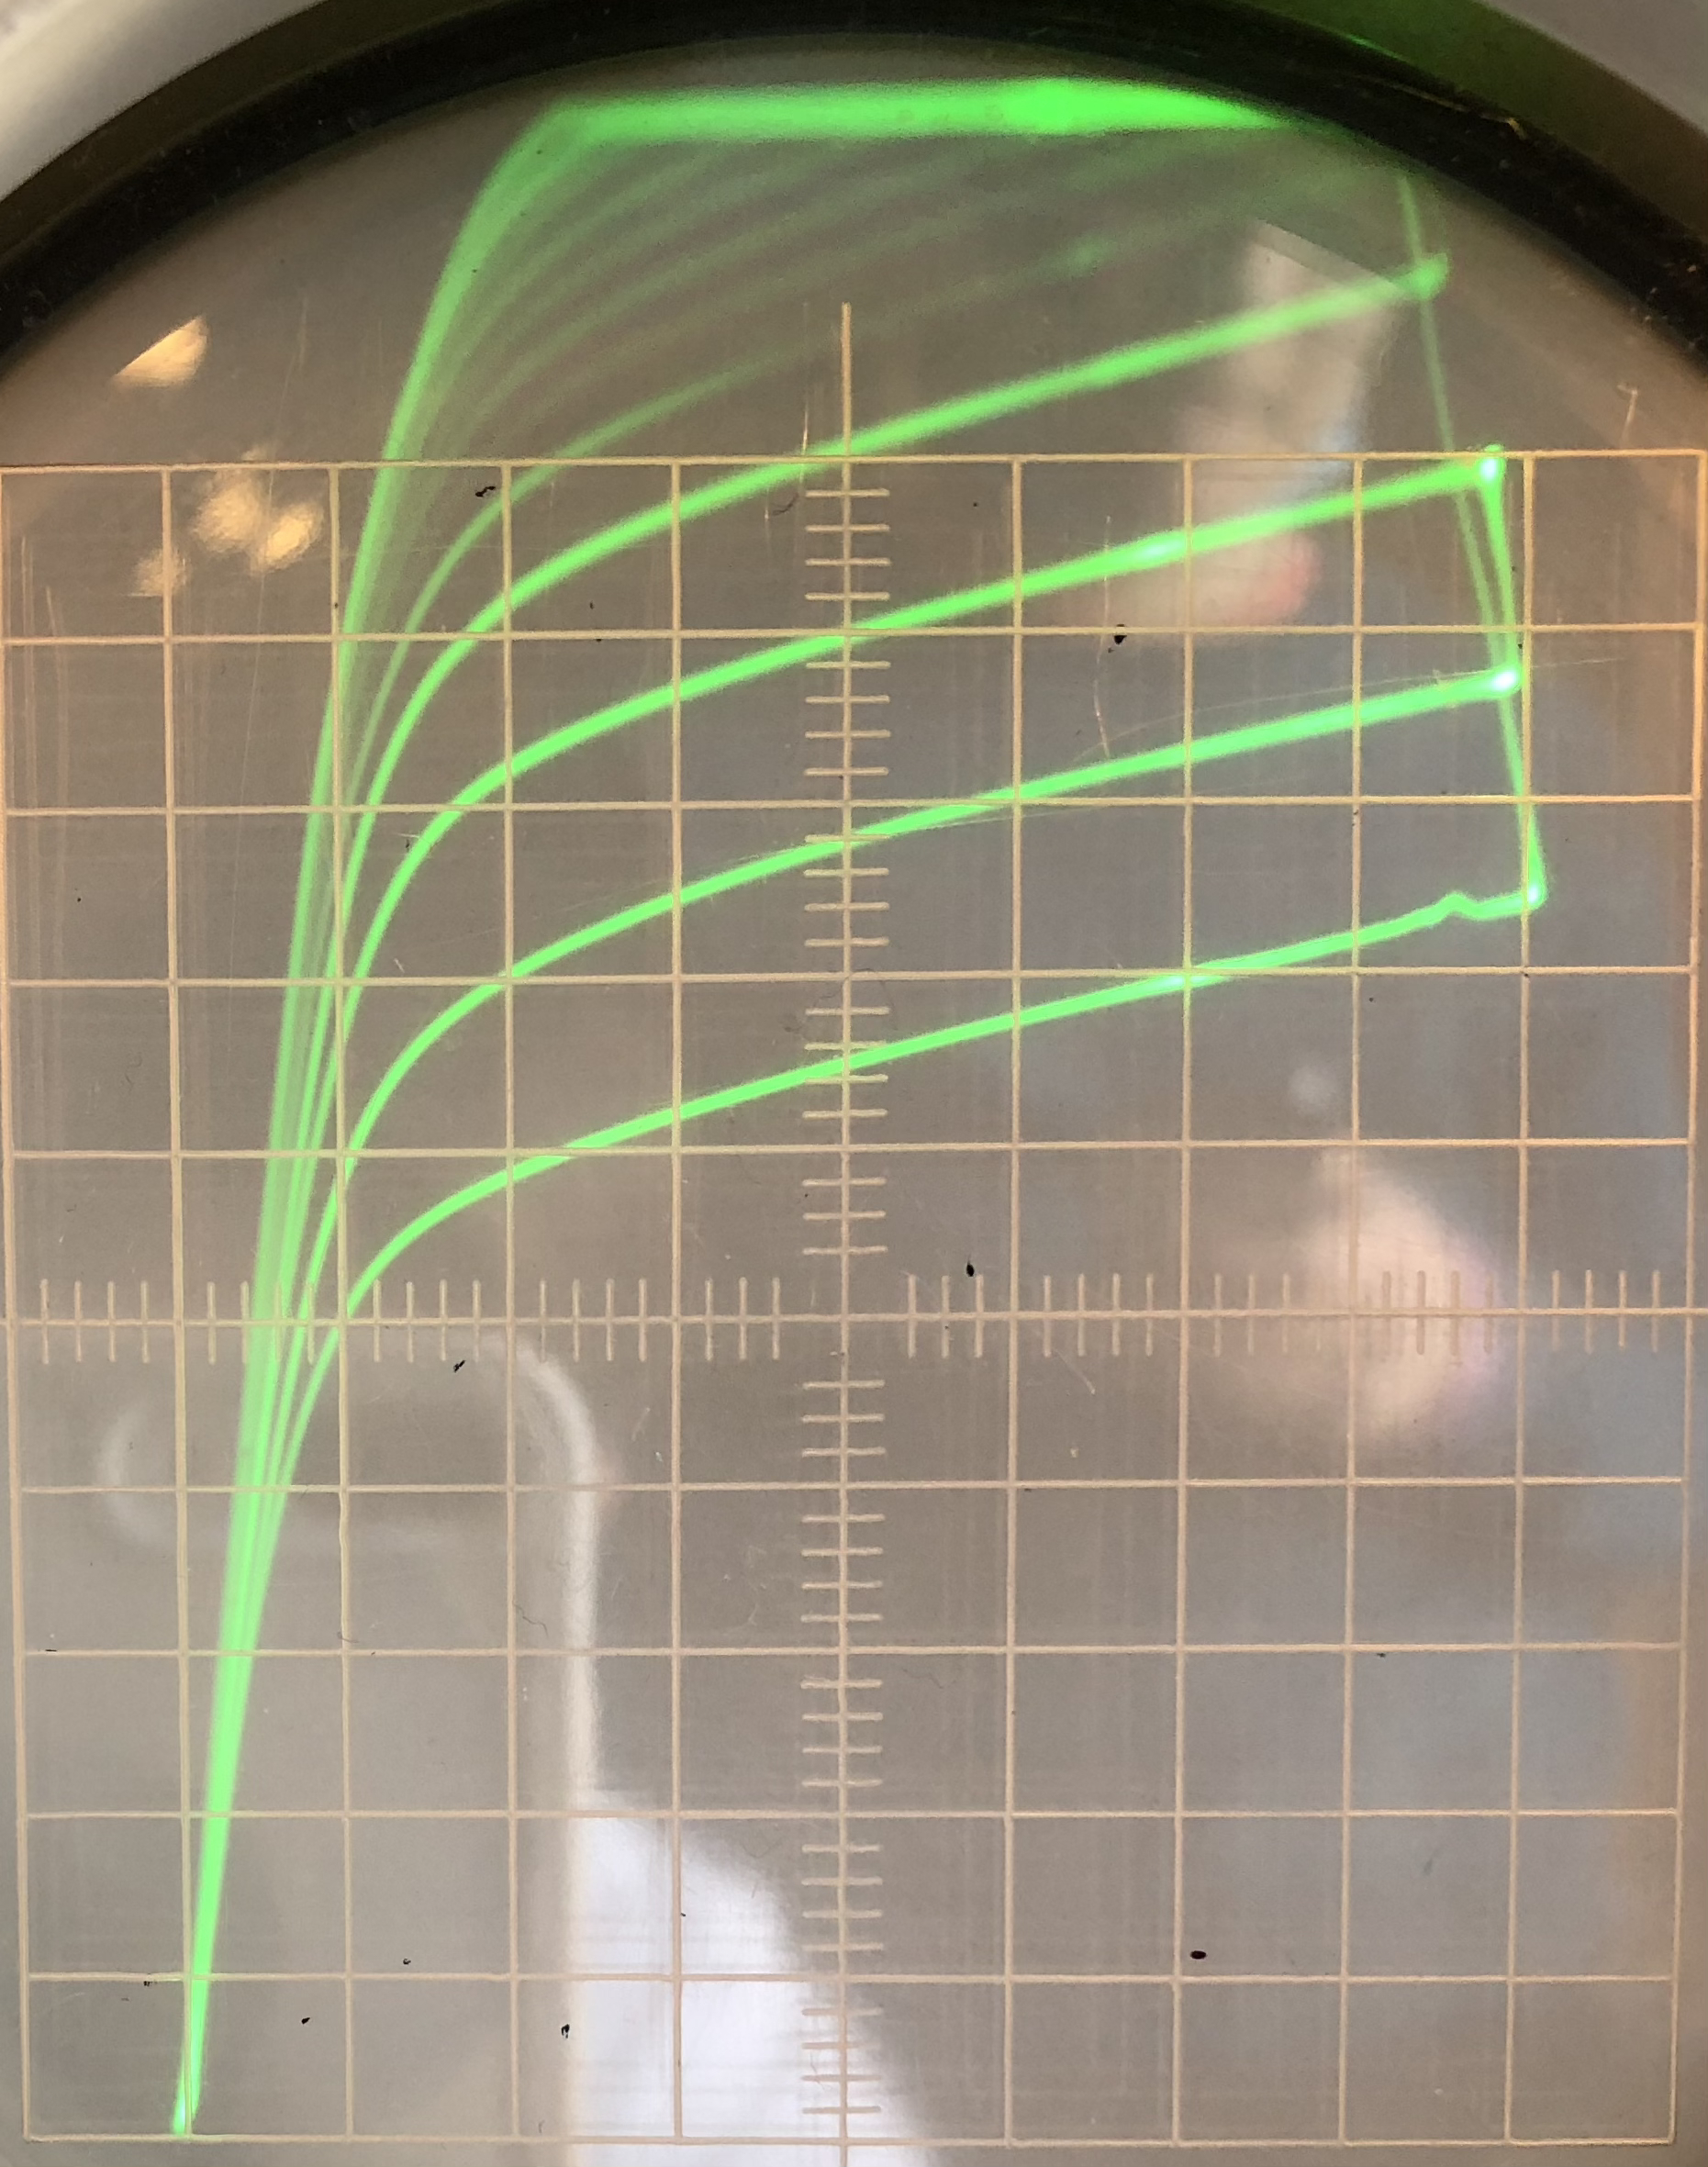
\includegraphics[width=1\linewidth]{p2.jpg}
        \caption{ВАХ при $V_з > 0$: X = +1 В, Y = +1 мА, Z = +0.2 В}
        \label{p2}
    \end{minipage}
    \end{center}
\end{figure}

\begin{enumerate}
    \item \textbf{Напряжение на затворе отрицательно $V_з < 0$} \par 

    \begin{itemize}
        \item  Определим запирающее напряжение на затворе. (рис. 1)

                \begin{center}
                    \fbox{$V_{зап} \approx  -1.9 \; В$}
                \end{center}

        \item Определим крутизну графика (рис. 1) в окресности точки $I_0 = 2.5\; мА$, $V_0 = 6\; В$:

            \begin{center}
                \fbox{$S = \frac{dI}{dV} \approx 5 \;  мА/В$}
            \end{center}

    \end{itemize}

    \item \textbf{Напряжение на затворе положительно $V_з > 0$} \par 
    Определим крутизну графика (рис. 2) в окресности точки $I_0 = 7.5\; мА$, $V_0 = 6\; В$:

    \begin{center}
        \fbox{$S = \frac{dI}{dV} \approx 6 \;  мА/В$}
    \end{center}

\end{enumerate}



	



\end{document}